\documentclass[aspectratio=169]{beamer}
\usetheme[]{metropolis}           % Use metropolis theme;
%\usepackage{FiraSans}

\usepackage{appendixnumberbeamer}
\usepackage[absolute,overlay]{textpos}
\usepackage[T1]{fontenc}
\usepackage{setspace}
\usepackage{xcolor}
\usepackage{caption}

%%%%%%%%%%%%%%%%%%%%%%%
% Background setup
\pgfdeclareimage[width=\paperwidth,height=\paperheight]{bg2}{figs/bg2} % Declare background image

\defbeamertemplate*{background canvas}{mydefault}
  {%
    \ifbeamercolorempty[bg]{background canvas}{}{\color{bg}\vrule width\paperwidth height\paperheight}% copied beamer default here
  }
  \defbeamertemplate*{background canvas}{bg}
 {%
   \color{mDarkTeal}\vrule width\paperwidth height\paperheight% added bg color
 }

 \defbeamertemplate*{background canvas}{image}
{%
    \begin{tikzpicture}
        \useasboundingbox (0,0) rectangle (\the\paperwidth, \the\paperheight);
        \pgftext[at=\pgfpoint{0cm}{0cm}, left, base]{\pgfuseimage{bg2}};
    \end{tikzpicture}
}

 \BeforeBeginEnvironment{frame}{%
   \setbeamertemplate{background canvas}[mydefault]%
 }

 \makeatletter
 \define@key{beamerframe}{bg}[true]{%
   \setbeamertemplate{background canvas}[bg]%
 }

\makeatletter
\define@key{beamerframe}{image}[true]{%
  \setbeamercovered{invisible}%
  \setbeamertemplate{background canvas}[image]%
}

%%%%%%%%%%%%%%%%%%%%%%
%% General setup
%% Fonts and typography
\setbeamerfont{title}{size=\huge,%
                      series=\bfseries}
\setbeamerfont*{subtitle}{size=\Large,%
                          series=\bfseries}
\setbeamerfont{author}{size=\large}
\setbeamerfont{date}{size=\large}
\setbeamerfont{frametitle}{size=\Large,%
                           series=\bfseries}

% color
\setbeamercolor{titlelike}{use=palette primary, parent=palette primary}
\setbeamercolor{author}{use=palette primary, parent=palette primary}
\setbeamercolor{date}{use=palette primary, parent=palette primary}
\setbeamercolor{institute}{use=palette primary, parent=palette primary}
\setbeamercolor{structure}{use=palette primary, parent=palette primary}

\setbeamertemplate{title}{
  \flushleft%
  \setstretch{.85}%
  \inserttitle%
  \par%
  \vspace*{0.1em}
 }
 \setbeamertemplate{subtitle}{
  \raggedright%
  \setstretch{.85}%
  \insertsubtitle%
  \par%
  \vspace*{0.5em}
}

% Title page frame
\setbeamertemplate{title page}{
%\pgfdeclareimage[height=0.6cm]{logo}{UdeS_blanc} % Declare first Logo
%\pgfdeclareimage[height=0.45cm]{logo2}{IELab} % Declare second Logo
  \begin{minipage}[b][\paperheight]{10cm}
    \ifx\inserttitlegraphic\@empty\else\usebeamertemplate*{title graphic}\fi
    \vfill%
    \ifx\inserttitle\@empty\else\usebeamertemplate*{title}\fi
    \ifx\insertsubtitle\@empty\else\usebeamertemplate*{subtitle}\fi
    %\usebeamertemplate*{title separator} % puts a line under the title
    \ifx\beamer@shortauthor\@empty\else\usebeamertemplate*{author}\fi
    \ifx\insertdate\@empty\else\usebeamertemplate*{date}\fi
    \ifx\insertinstitute\@empty\else\usebeamertemplate*{institute}\fi
    %\vfill%
    \vspace*{8mm}
    %\pgfuseimage{logo} % Use logo
    %\newcommand\mybar{\kern1pt\rule[-\dp\strutbox]{.8pt}{.7cm}{\hspace{2mm}}\kern1pt} % White bar
    %\textcolor{white}{\mybar{\pgfuseimage{logo2}}} % Second logo
    %\vfill
    \vspace*{15mm}
  \end{minipage}
}

%%%%%%%%%%%%%%%%%%%%%%%%%%%
% Examples

%% Makes title slide with only background defined color
  %\begin{frame}[bg]
    %\titlepage
  %\end{frame}
%% Makes a title slide with background + image
  %\begin{frame}[image]
    %\titlepage
  %\end{frame}
%% Makes also a title slide with background + image
  %\maketitle

%%%%%%%%%%%%%%%%%%%%%%%%%%%

\title{Aire de distribution et changements climatiques:}
\subtitle{Comment les interactions biotiques moduleront-elles la réponse?}
%\date{\today}
\author{Victor Cameron}




\begin{document}

%% Effect of climate change on the co-distribution of forest trees and passerine birds
\maketitle % make title produces formated title slide

%%% keys
%1. Le titre
%2. Structure spéciale: Étude théorique = exploration
%3. Pas d'hypothèse
%4. Cette présentation a pour but de présenter mon projet

%%%%%%%%%%%%%%%%%%%%%%%%%%%%%%%%%%%%%%%%%%%%%%%%%%%%%%%%%%%%%%%%%%%%%%%%%%%%%%%%%
%%% Contexte

{%
\setbeamertemplate{frame footer}{Ferrarini \textit{et al}. 2017}
\begin{frame}{Contexte\hskip 1em \mdseries{\textcolor{lightgray}{Les limites de distribution}}}

  Un \textbf{déplacement des aires de distribution} est attendu dans les 100 prochaines années

  \begin{figure}
  	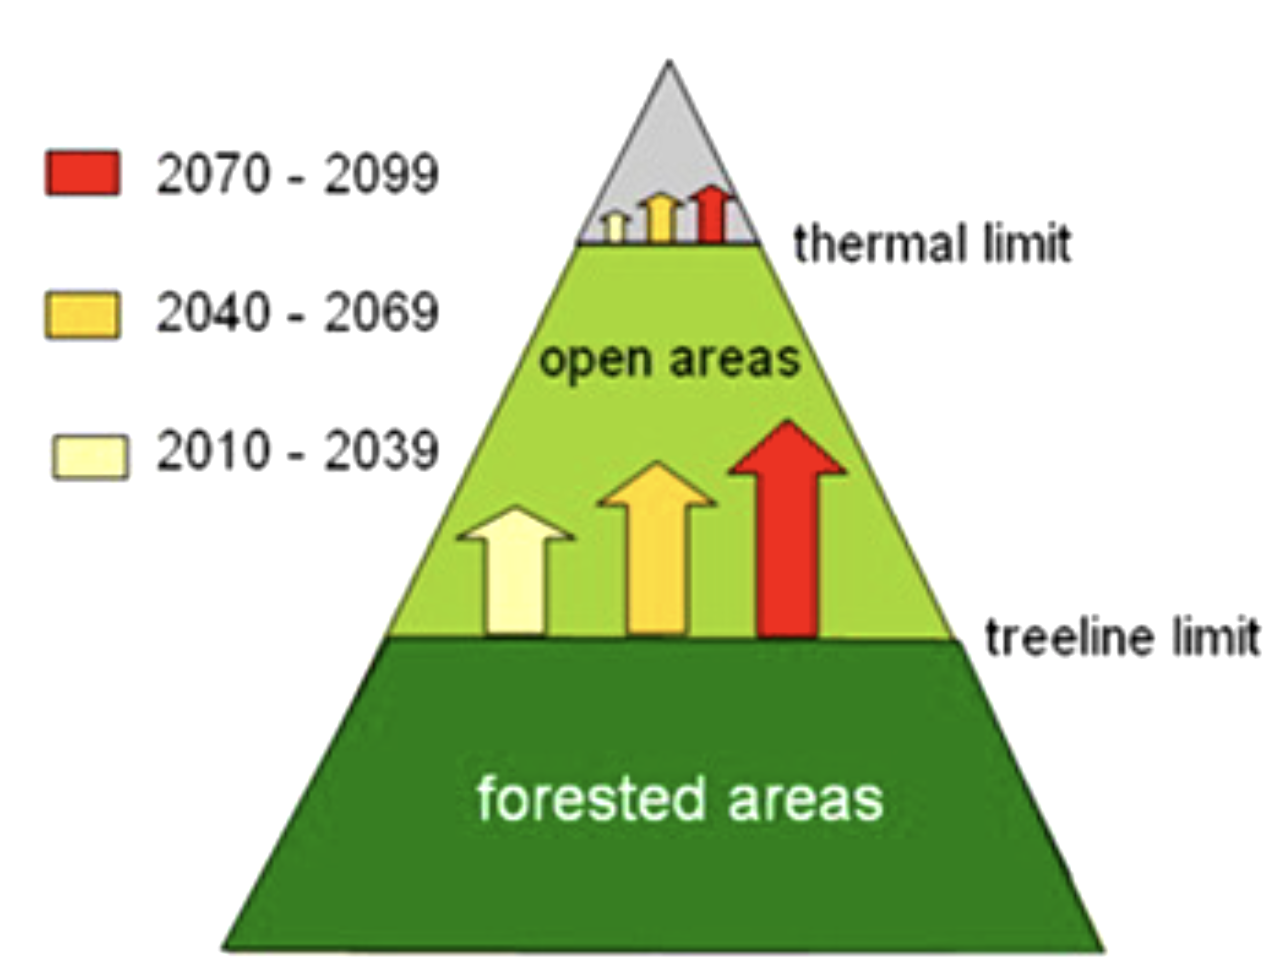
\includegraphics[height=.60\paperheight]{figs/Ferrarini.png}
    %\caption*{ \textbf{Eveloppe climatique de l'érable à sucre présente et projetée (2071-2100)}}
  \end{figure}

\end{frame}
}

%%% L'aire de distribution d'une espèce est limitée
%%% Une connaissance des processus limitant l'aire de distribution est fondamentale pour prévoir les distributions dans le futur

%%%%%%%%%%%%%%%%%%%%%%%%%%%%%%%%%%%%%%%%%%%%%%%%%%%%%%%%%%%%%%%%%%%%%%%%%%%%%%%%%
%%% Contexte

{%
\setbeamertemplate{frame footer}{}
\begin{frame}{Contexte\hskip 1em \mdseries{\textcolor{lightgray}{Les limites de distribution}}}

  1. L'emplacement des limites de distribution est \textbf{sensible au climat}

  \begin{figure}
  	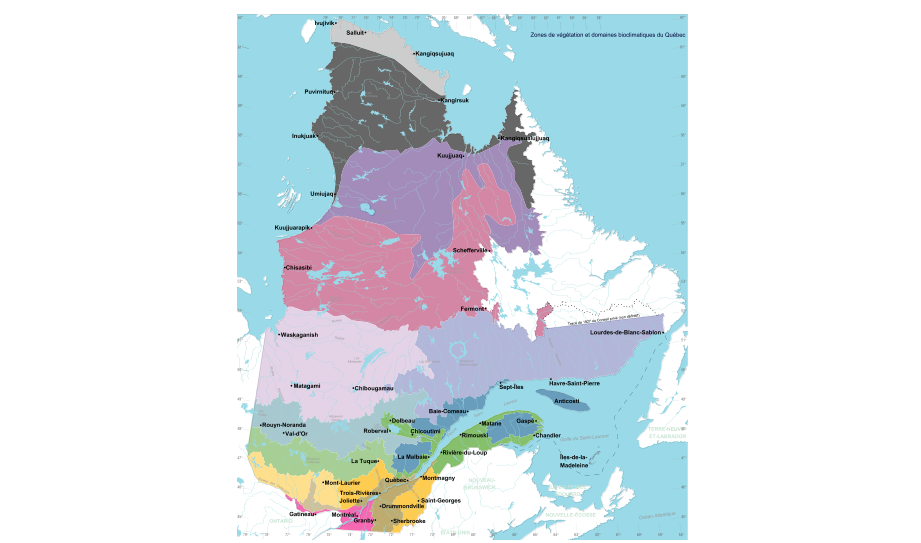
\includegraphics[height=.65\paperheight]{figs/bioclim.png}
    %\caption*{ \textbf{Distribution présente et projetée}}
  \end{figure}

\end{frame}
}

%%% On s'attend à trouver les espèces là où le climat est favorable et absentes là où le climat est défavorable
%%%

%%%%%%%%%%%%%%%%%%%%%%%%%%%%%%%%%%%%%%%%%%%%%%%%%%%%%%%%%%%%%%%%%%%%%%%%%%%%%%%%%
%%% Contexte

{%
\setbeamertemplate{frame footer}{}
\begin{frame}{Contexte\hskip 1em \mdseries{\textcolor{lightgray}{Projection des futures distributions}}}

  2. On s'attend à ce que les enveloppes climatiques se \textbf{déplacent vers le nord ou vers des altitudes plus élevées} en réponse aux changements climatiques

  \begin{figure} % Photos de passeraux associés à divers types de forêts
    % Paruline azurée (ou couronnée?) est associée aux érablières
    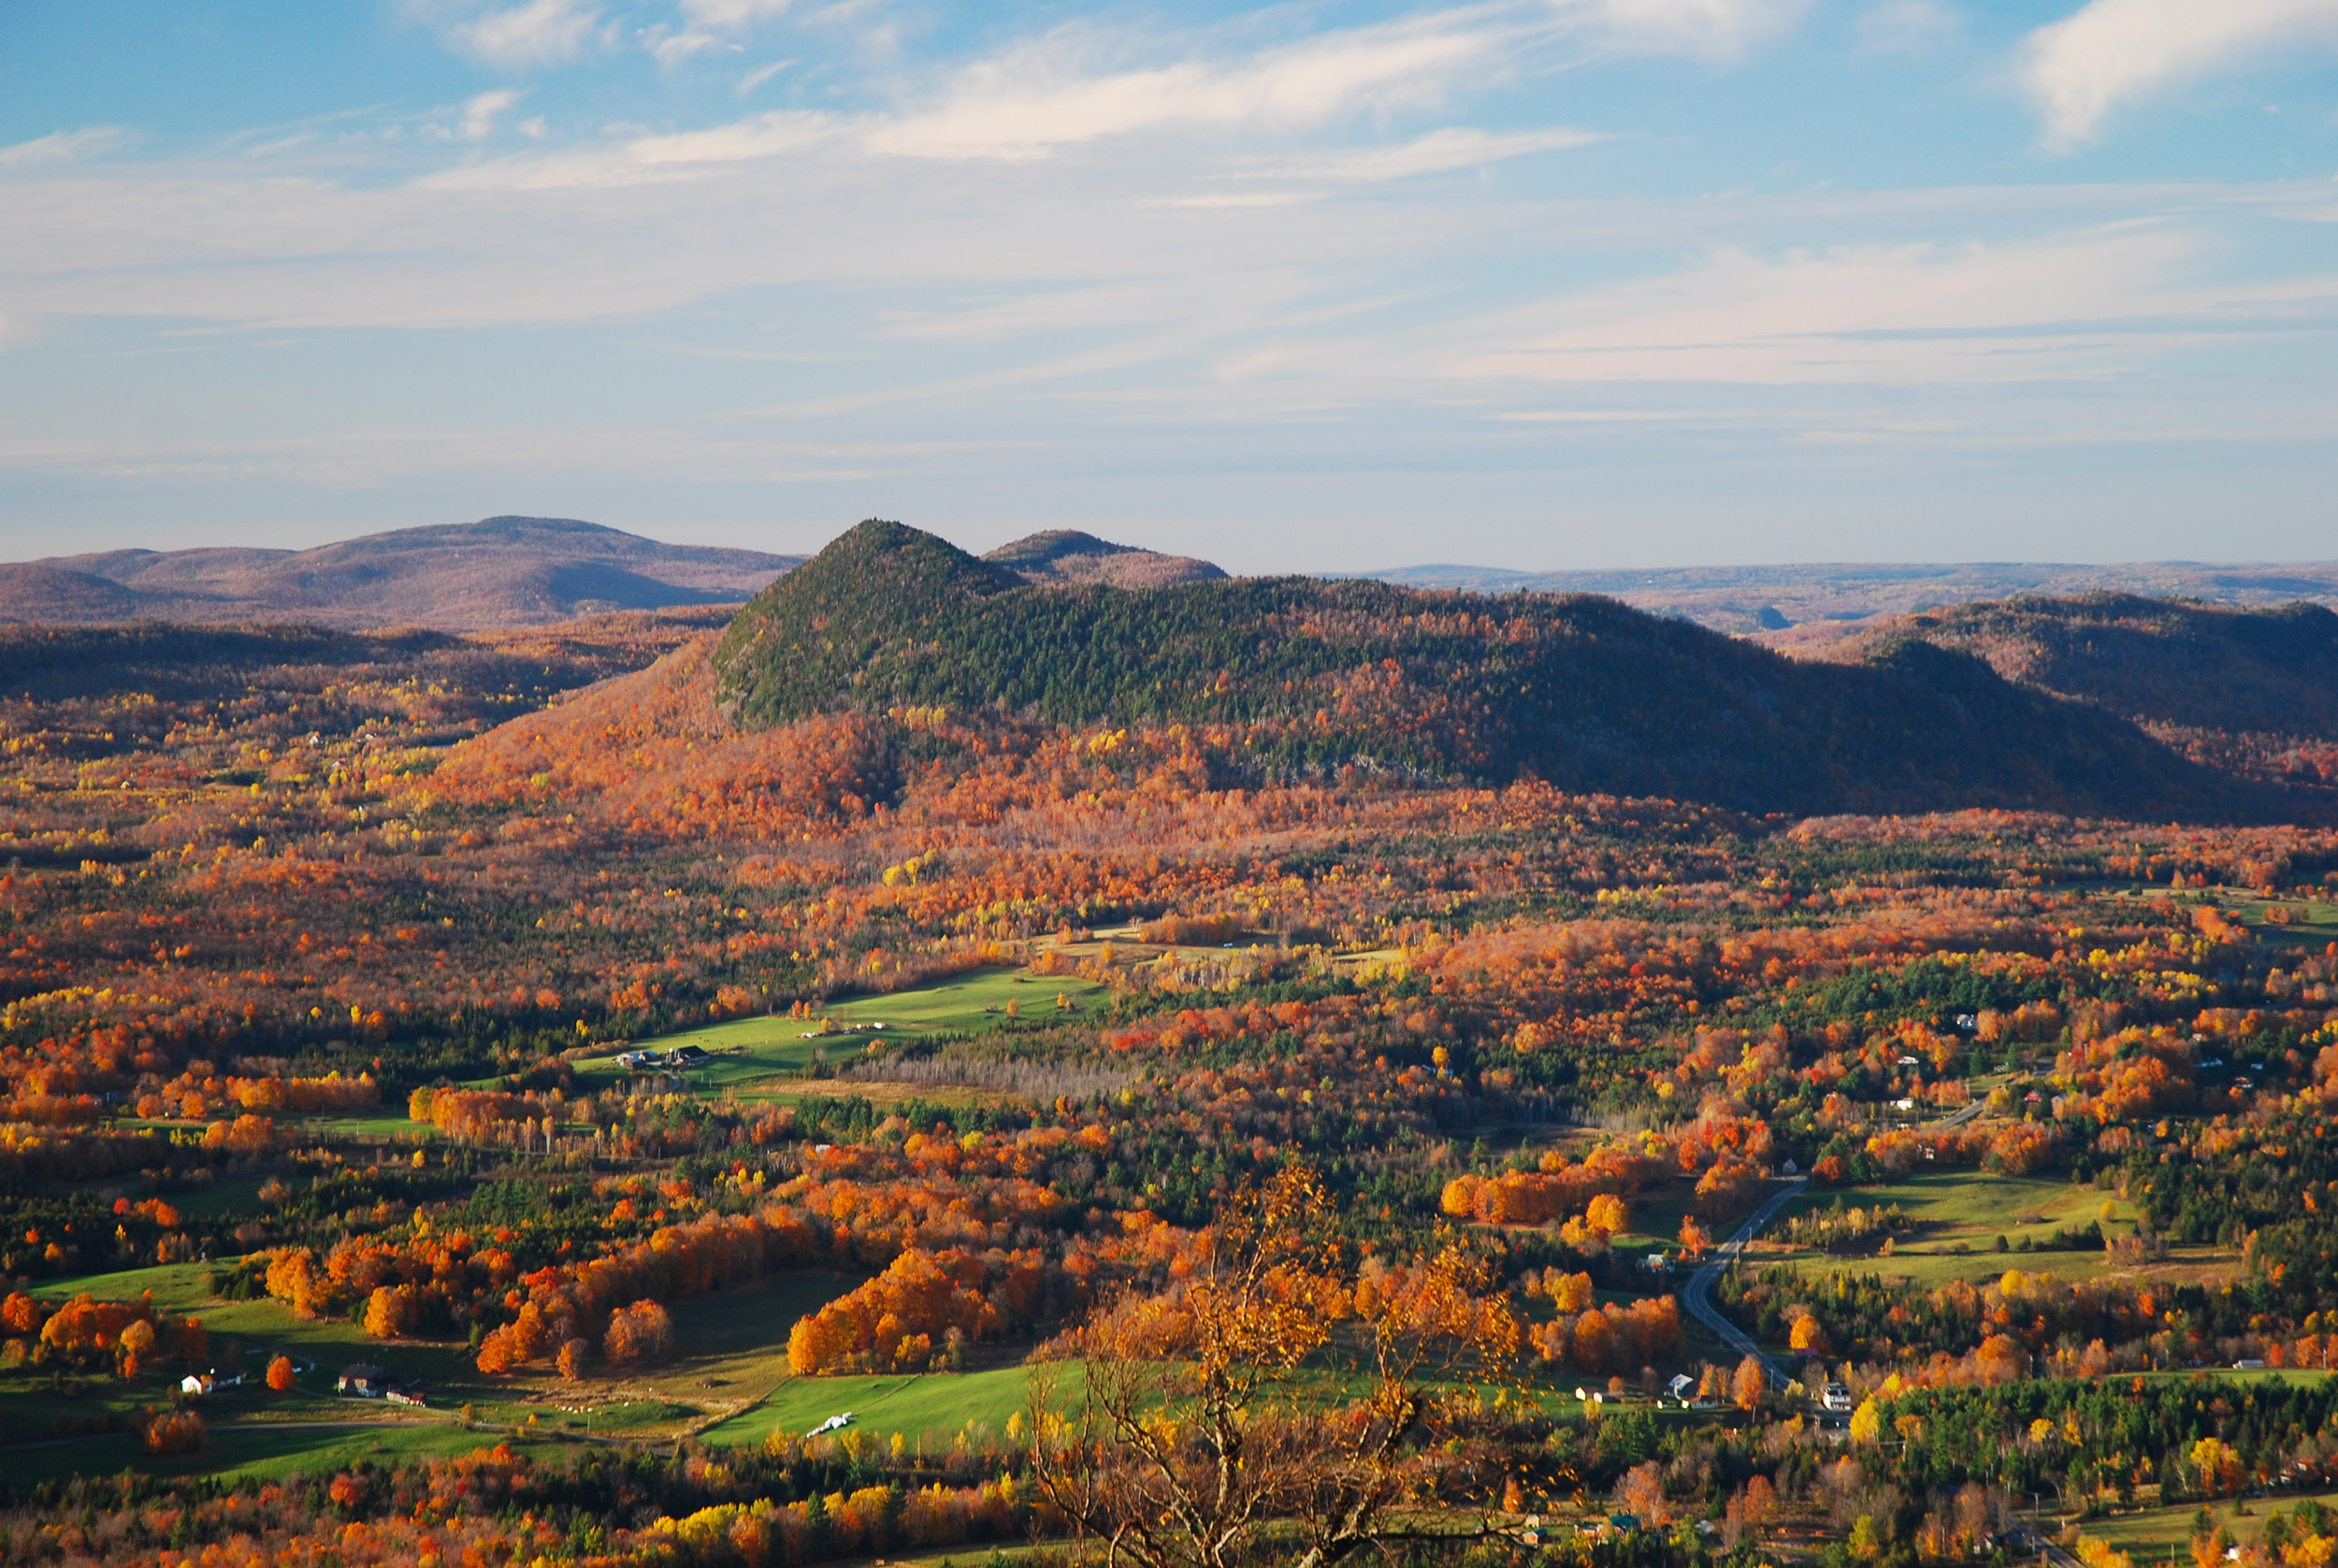
\includegraphics[width=0.5\textwidth]{figs/corridor.jpg}

  \end{figure}

\end{frame}
}

%%% Les espèces réactives pourront suivre le déplacement de leur enveloppe climatique
%%% Les espèces moins réactives accuseront un retard
%%% Il a été observé que la végétation accuse un retard sur le déplacement son enveloppe climatique
%%% Différents temps de réactions peuvent faire que des espèces qui co-occurent présentement ne co-occurent plus dans le futur

%%%%%%%%%%%%%%%%%%%%%%%%%%%%%%%%%%%%%%%%%%%%%%%%%%%%%%%%%%%%%%%%%%%%%%%%%%%%%%%%%
%%% Contexte

{%
\setbeamertemplate{frame footer}{McKenney \textit{et al}. 2007, Talluto \textit{et al}. 2017}
\begin{frame}[t]{Contexte\hskip 1em \mdseries{\textcolor{lightgray}{Difficultés reliées au contexte}}}

  Les \textbf{modèles de distribution d'espèces} (SDMs) sont des modèles mathématiques qui corrèlent la \emph{distribution} d'une espèce avec des \emph{données climatiques}

  \begin{columns}[]
    \begin{column}{0.5\textwidth}
      \begin{figure}
        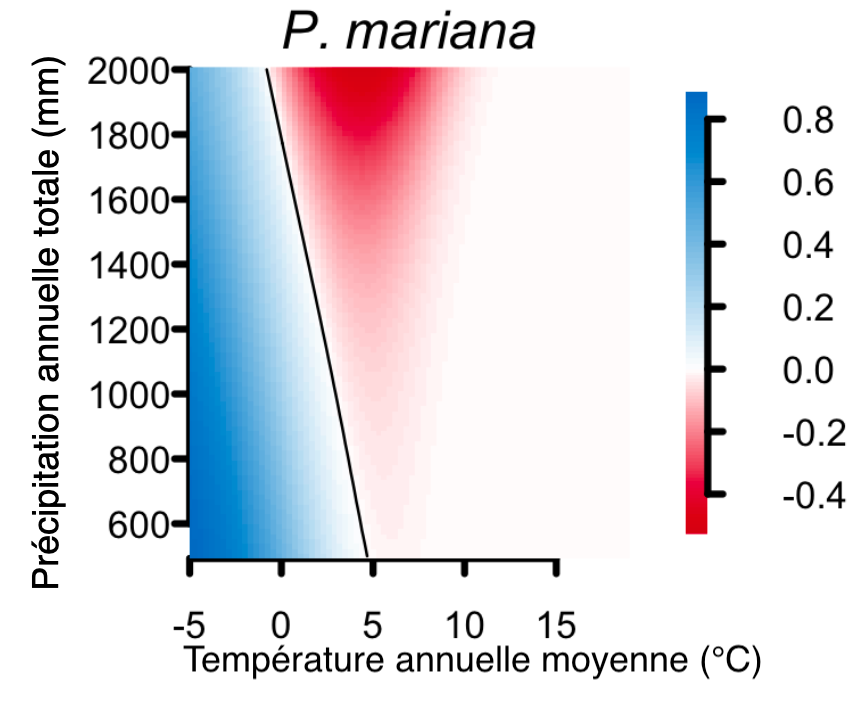
\includegraphics[height=.65\textwidth]{figs/Talluto2.png}
      \end{figure}
    \end{column}

    \begin{column}{0.5\textwidth}
      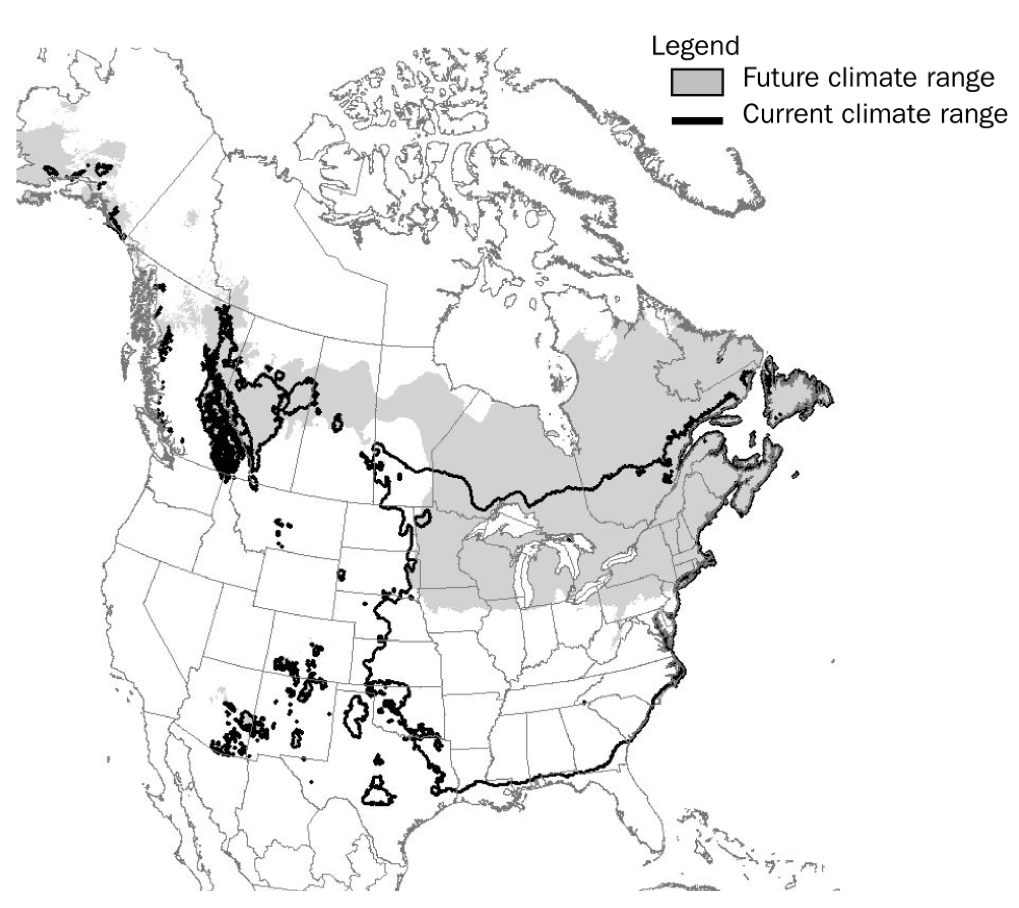
\includegraphics[height=.65\textwidth]{figs/mckenney.png}
    \end{column}
  \end{columns}

\end{frame}
}

%% Les SDMs sontdes modèles mathématiques

%%%%%%%%%%%%%%%%%%%%%%%%%%%%%%%%%%%%%%%%%%%%%%%%%%%%%%%%%%%%%%%%%%%%%%%%%%%%%%%%%
%%% Contexte

\begin{frame}{Contexte\hskip 1em \mdseries{\textcolor{lightgray}{Difficultés reliées au contexte}}}

  Les \textbf{modèles de distribution d'espèces} (SDMs) font de nombreuses suppositions:
    \begin{itemize}
      \item Distribution à l'équilibre avec l'enveloppe climatique;
      \item Absence de démographie;
      \item Absence de limite de dispersion;
      \item Absence d'interaction biotique;
      \item Réponse linéaire et instantannée au changement climatique.
    \end{itemize}

\end{frame}

%% Les outils actuels pour prédire l'impact des changements climatiques sur la distribution des espèces sont limités par l'absence de processus écologiques fondamentaux.
%% Def interaction: l'effet qu'une espèce  a sur le fitness d'une autre espèce (taux de croissance de population): pred-proie, habitat-utilisateur

%%%%%%%%%%%%%%%%%%%%%%%%%%%%%%%%%%%%%%%%%%%%%%%%%%%%%%%%%%%%%%%%%%%%%%%%%%%%%%%%%
% % % Contexte

\begin{frame}{Contexte\hskip 1em \mdseries{\textcolor{lightgray}{Difficultés reliées au contexte}}}

  %% Quand on s'intéresse au changements d'aire de répartition d'une communauté, certains processus sont à prendre en considérations:
  Les espèces qui \textbf{co-occurent}:
  \begin{itemize}
    \item Ont différents temps de réponse au changement climatique;
    \item Ne se reproduisent pas au même rythme;
    \item N'ont pas toutes la même capacité de dispersion;
    \item Interagissent.
  \end{itemize}

  \alert{Ces processus peuvent modifier la relation entre le climat et la distribution des espèces}

\end{frame}

%% Les processus peuvent avoir des conséquences inatendues sur les futures distributions

%%%%%%%%%%%%%%%%%%%%%%%%%%%%%%%%%%%%%%%%%%%%%%%%%%%%%%%%%%%%%%%%%%%%%%%%%%%%%%%%%
% % %

\begin{frame}{Objectifs\hskip 1em \mdseries{\textcolor{lightgray}{Subtitle}}}

  \textbf{Objectif général:} Évaluer les impacts d'un changement climatique sur la distribution régionale et la persistance d'une espèce en intéraction avec son habitat.

  \textbf{\\Objectifs secondaires:}
  \begin{enumerate}
    \item Développer un nouvel outil théorique pour améliorer la prédiction des impacts du changement climatique sur la distribution des espèces;
    \item Évaluer l'impact des interactions biotiques sur la réaction des aires de distribution au changement climatique.
  \end{enumerate}

\end{frame}

%%%%%%%%%%%%%%%%%%%%%%%%%%%%%%%%%%%%%%%%%%%%%%%%%%%%%%%%%%%%%%%%%%%%%%%%%%%%%%%%%
% % %

{%
\setbeamertemplate{frame footer}{Pulliam 2000, Sandoro 2008}
\begin{frame}{Théorie \hskip 1em \mdseries{\textcolor{lightgray}{Interactions biotiques}}}

Les \textbf{interactions biotiques} sont d'importantes forces modulaires des limites de distribution à \emph{petites et à grandes échelles spatiales}

\begin{figure}
  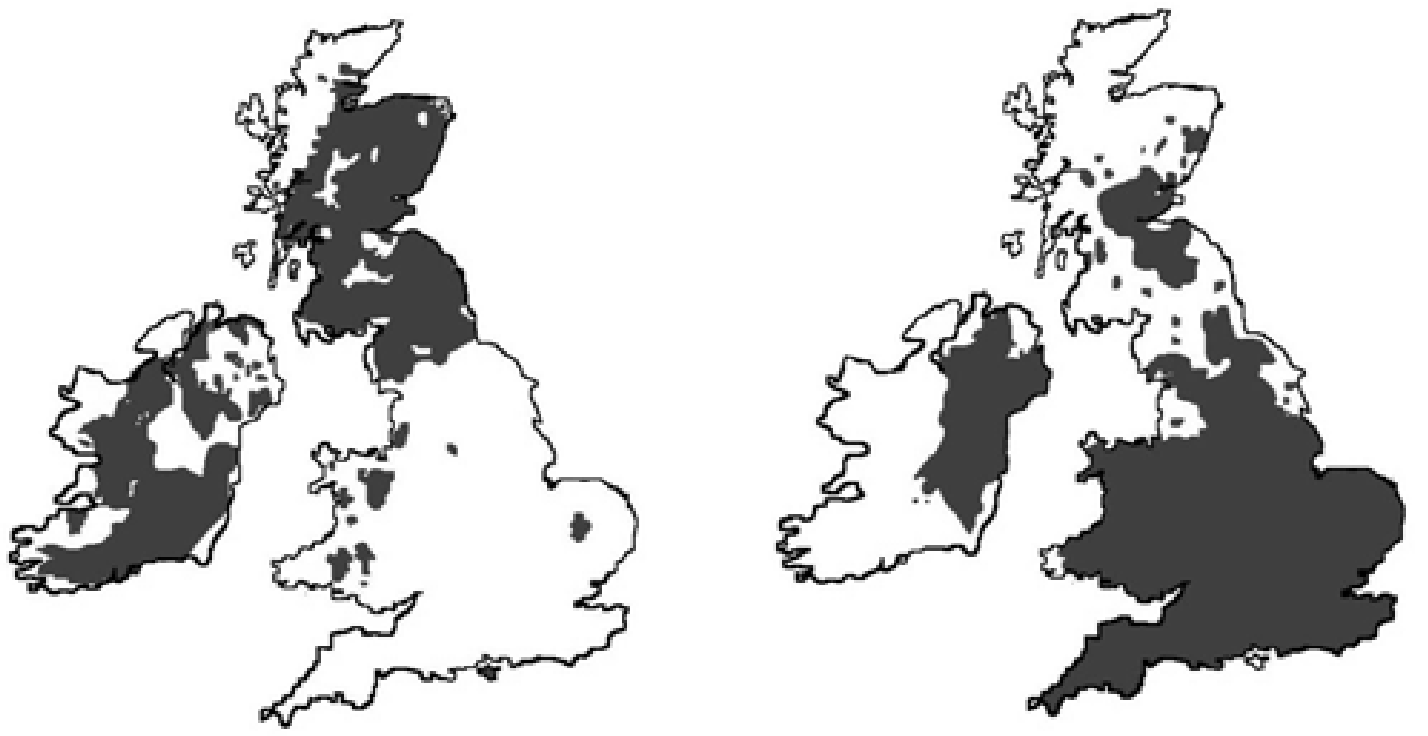
\includegraphics[height=.60\paperheight]{figs/Sandoro.png}
  %\caption*{ \textbf{}}
\end{figure}

\end{frame}
}

%% Interaction biotiques: effet d'une espèce sur le fitness (taux de croissance) d'une autre espèce
%% Historiquement: Conditions climatiques importantes à large échelle, et les interactions à l'échelle locale
%% Little interest in the study of biotic interactions at large geographical scales: important need for methods to account for interactions in future predictions

%%%%%%%%%%%%%%%%%%%%%%%%%%%%%%%%%%%%%%%%%%%%%%%%%%%%%%%%%%%%%%%%%%%%%%%%%%%%%%%%%
% % %

{%
\setbeamertemplate{frame footer}{Pulliam 2000, Godsoe \textit{et al}. 2017}
\begin{frame}{Théorie\hskip 1em \mdseries{\textcolor{lightgray}{La niche écologique}}}
  La \textbf{niche fondamentale} fait référence aux \emph{conditions climatiques}: là où l'espèce \emph{peut} être présente
  \begin{equation*}
    \underbrace{r(E)}_{\text{croissance}} > \underbrace{b(E)}_{\text{naissances}} - \underbrace{d(E)}_{\text{mortalité}}
  \end{equation*}

  \begin{columns}[]
    \begin{column}{0.5\textwidth}
      \begin{figure}
        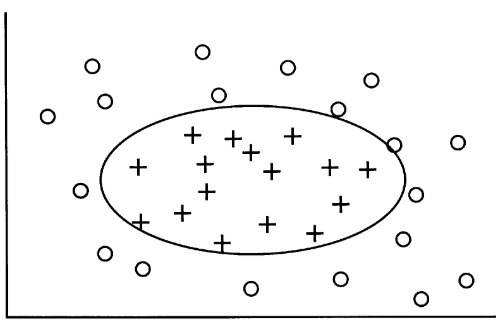
\includegraphics[width=0.8\textwidth]{figs/puliam1.png}
      \end{figure}
    \end{column}

    \begin{column}{0.5\textwidth}
      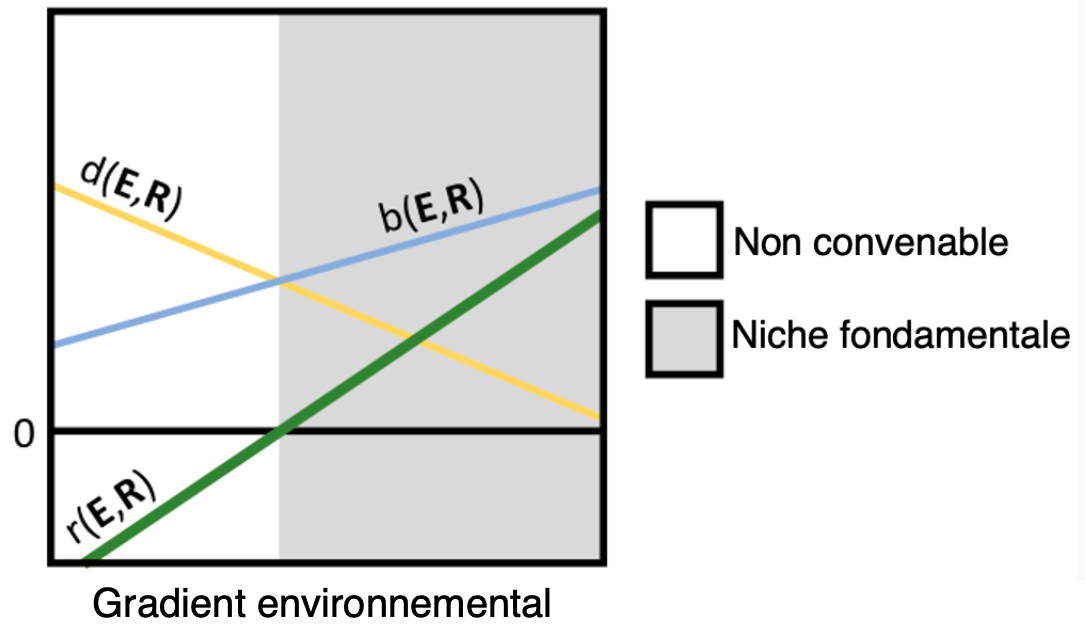
\includegraphics[width=0.95\textwidth]{figs/godsoe1.png}
    \end{column}
  \end{columns}

\end{frame}
}

%% Godsoe: approche les limites de distribution avec la théorie de la niche (r>b-d)
%% Besoin d'une perspective régionale (\lambda>c-e --> suget de ma maitrise (montrer les schémas que j'ai fait)

%%%%%%%%%%%%%%%%%%%%%%%%%%%%%%%%%%%%%%%%%%%%%%%%%%%%%%%%%%%%%%%%%%%%%%%%%%%%%%%%%
% % %

{%
\setbeamertemplate{frame footer}{Pulliam 2000, Godsoe \textit{et al}. 2017}
\begin{frame}{Théorie\hskip 1em \mdseries{\textcolor{lightgray}{La niche écologique}}}

  %b,d --> c,e,h  (disponibilité d'habitat: montrer schéma que j'ai fait)
  La \textbf{niche réalisée} fait référence aux \emph{conditions climatiques et autres facteurs}: là où l'espèce \emph{est} présente
  \begin{equation*}
    \underbrace{r(E)}_{\text{croissance}} > \underbrace{b(E)}_{\text{naissances}} - \underbrace{d(E)}_{\text{mortalité}} + \underbrace{I(E)}_{\text{interactions}}
  \end{equation*}

  \begin{columns}[]
    \begin{column}{0.5\textwidth}
      \begin{figure}
        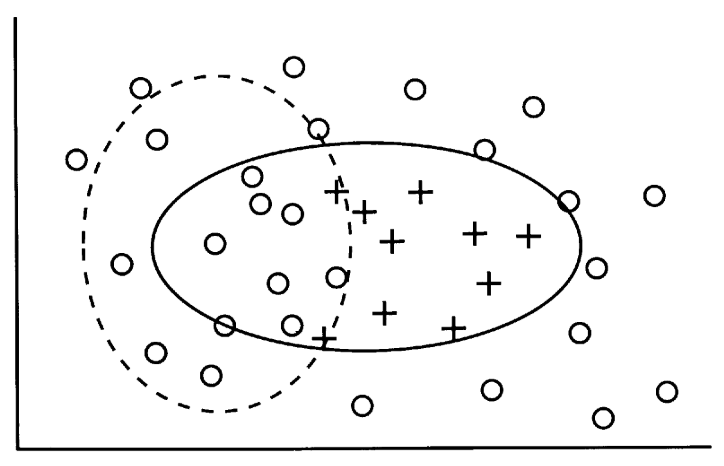
\includegraphics[width=0.75\textwidth]{figs/pulliam2.png}
      \end{figure}
    \end{column}

    \begin{column}{0.5\textwidth}
      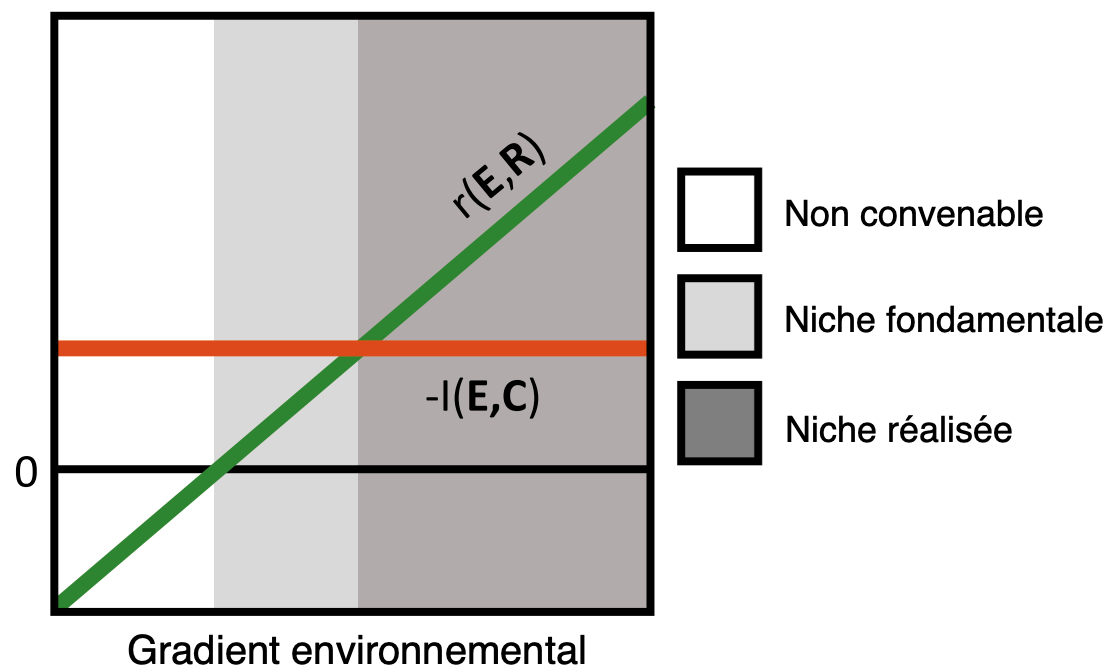
\includegraphics[width=.95\textwidth]{figs/godsoe2.png}
    \end{column}
  \end{columns}

\end{frame}
}

%% Besoin d'une perspective régionale (\lambda>c-e --> suget de ma maitrise (montrer les schémas que j'ai fait)
%% disponibilité d'habitat

%%%%%%%%%%%%%%%%%%%%%%%%%%%%%%%%%%%%%%%%%%%%%%%%%%%%%%%%%%%%%%%%%%%%%%%%%%%%%%%%%
% % %

{%
\setbeamertemplate{frame footer}{Schooley and Consentino 2018}
\begin{frame}{Théorie\hskip 1em \mdseries{\textcolor{lightgray}{Métapopulations}}}

  \begin{columns}
    \begin{column}{0.5\textwidth}
      \begin{equation*}
          \frac{dP}{dt} = c(h-P) - eP
      \end{equation*}
    \end{column}

    \begin{column}{0.5\textwidth}
      \begin{equation*}
        h > \frac{e}{c}
      \end{equation*}
    \end{column}
  \end{columns}

  \begin{figure}
    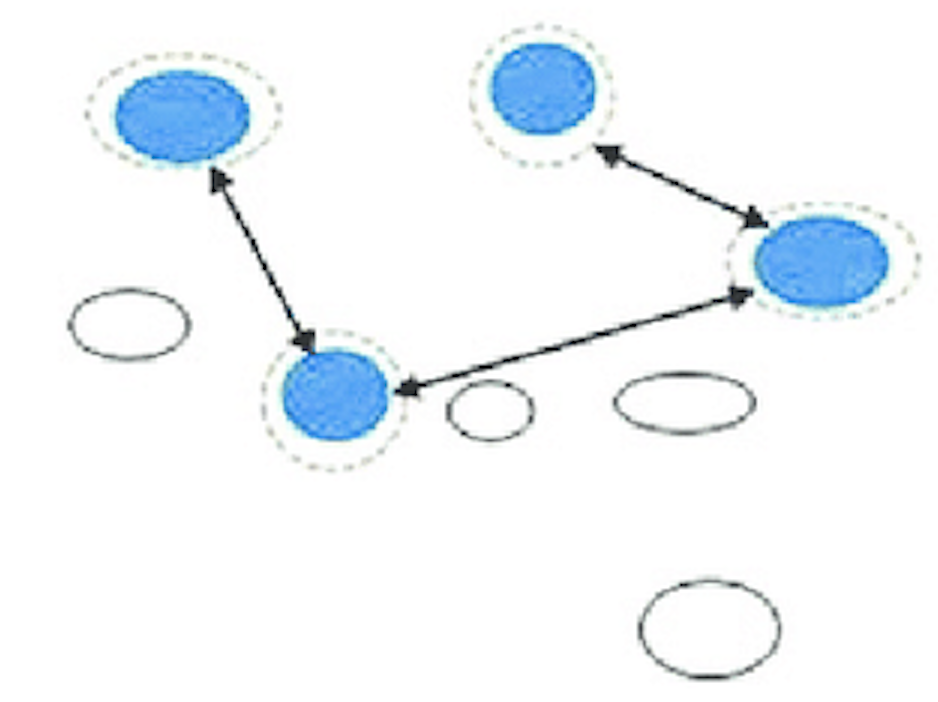
\includegraphics[width=.60\paperheight]{figs/metapop.png}
  \end{figure}

\end{frame}
}

%% Besoin d'une perspective régionale (\lambda>c-e --> suget de ma maitrise (montrer les schémas que j'ai fait)
%% h: disponibilité d'habitat
%% h>e/c --> condition de la distribution d'une espèce; h=e/c ou c*h=e est la limite de distribution

%%%%%%%%%%%%%%%%%%%%%%%%%%%%%%%%%%%%%%%%%%%%%%%%%%%%%%%%%%%%%%%%%%%%%%%%%%%%%%%%%
% % %

\begin{frame}{Théorie\hskip 1em \mdseries{\textcolor{lightgray}{Métapopulations}}}

  \begin{equation*}
    \textcolor{lightgray}{\underbrace{b(E)}_{\text{naissances}} = \underbrace{d(E)}_{\text{mortalité}}}
  \end{equation*}

  \begin{equation*}
    \underbrace{c(E)}_{\text{colonisations}} * \underbrace{h}_{\text{disponibilité d'habitat}} = \underbrace{e(E)}_{\text{extinctions}}
  \end{equation*}

\end{frame}

%% Une population est une patch individuelle, une métapopulation est un amalgame de plusieurs patchs
%% À l'échelle régionale, la distribution d'une espèce est l'ensemble des regions où une espèce est présente

%%%%%%%%%%%%%%%%%%%%%%%%%%%%%%%%%%%%%%%%%%%%%%%%%%%%%%%%%%%%%%%%%%%%%%%%%%%%%%%%%
% % %

\begin{frame}{Théorie\hskip 1em \mdseries{\textcolor{lightgray}{Métapopulations}}}

  La \textbf{capacité de support} d'une métapopulation est une mesure de viabilité de l'espèce
  $$\lambda > \frac{e}{c}$$
  \begin{figure}
    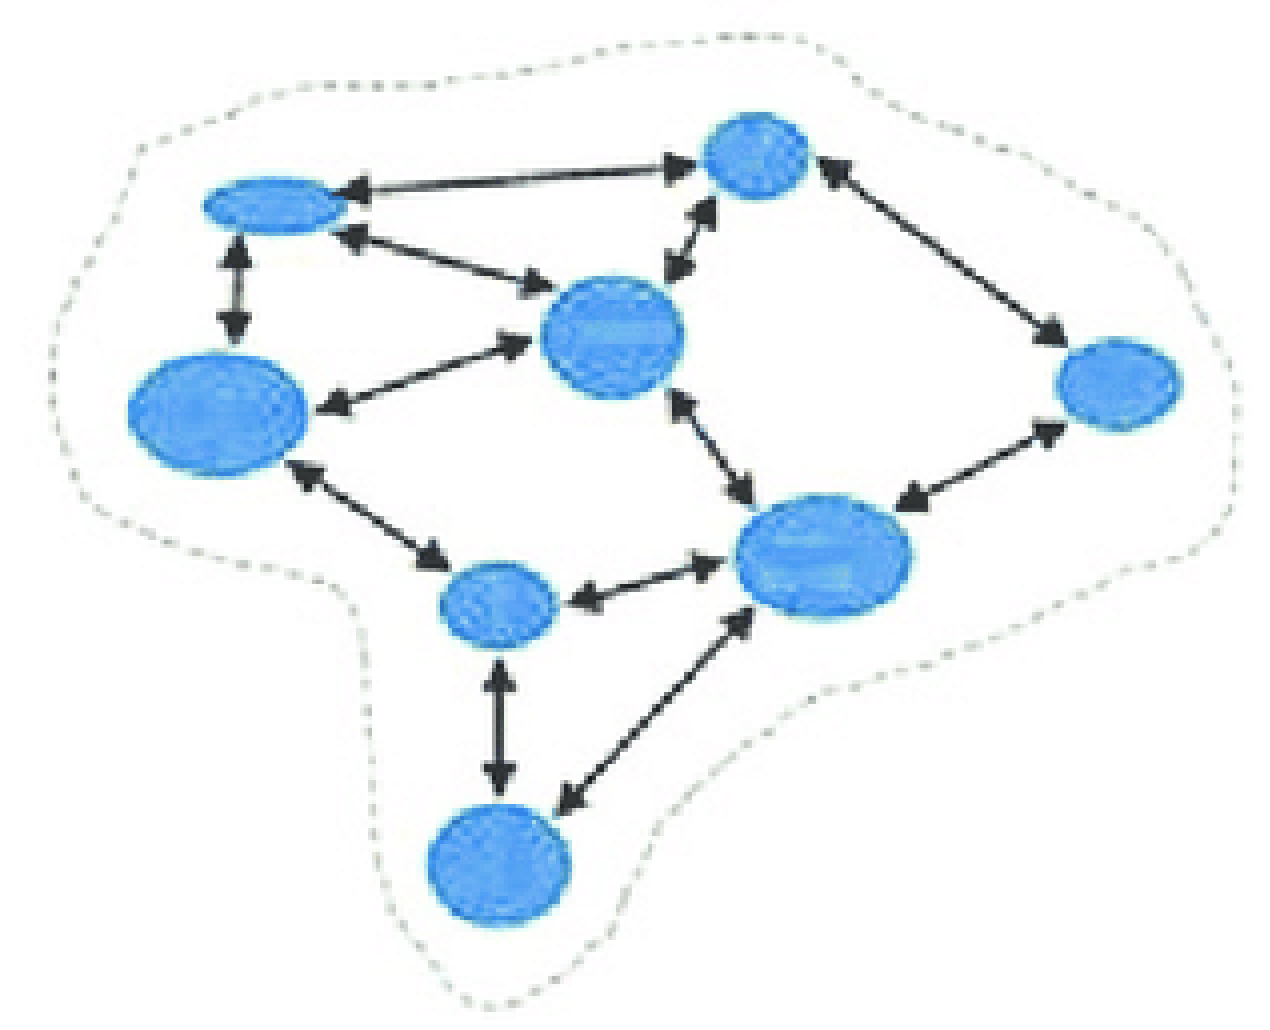
\includegraphics[width=.60\paperheight]{figs/metapop2.png}
  \end{figure}

\end{frame}

%% La capacité de support est en quelque sorte une mesure du risque d'extinction de l'espèce; c'est une mesure de la structure de l'habitat (# patch, aire des patch; distances) tel qu'expérimenté par l'espèce sur sa persistence
%% Intéressent pour mesurer l'impact d'un changement climatique sur une espèce à l'échelle régionale; différence dans la viabilité
%% Intéressent pour mesurer l'impact des interactions sur la réponse espèce à l'échelle régionale; différence dans le risque d'extinction avant-après
%% La capacité de support d'une métapopulation est l'équilibre entre les estinctions locales et les colonisations de patch vides
%% Pour une métapopulation réaliste (spatiale) qui représente un paysage, la persistence est défénie par la structure du paysage

%%%%%%%%%%%%%%%%%%%%%%%%%%%%%%%%%%%%%%%%%%%%%%%%%%%%%%%%%%%%%%%%%%%%%%%%%%%%%%%%%
% % %

\begin{frame}{Étude de cas\hskip 1em \mdseries{\textcolor{lightgray}{Les Appalaches}}}

  Pour aider à relier les concepts que j'ai presenté et les objectifs que je me suis fixés

  \begin{figure}
  	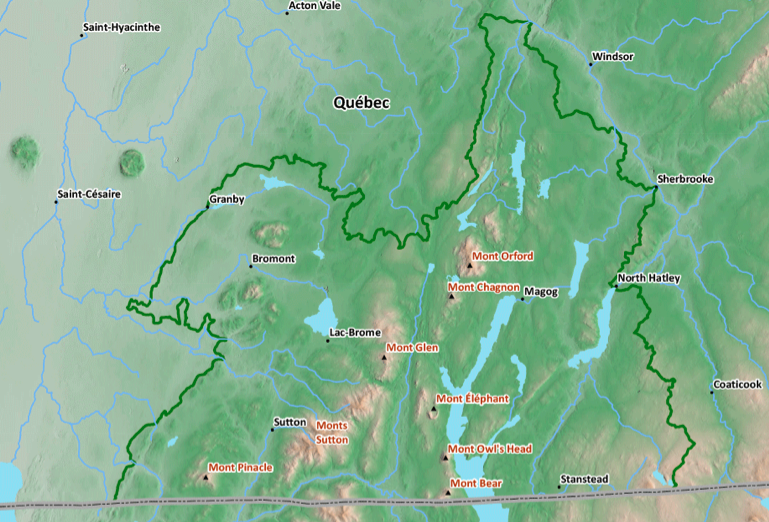
\includegraphics[height=.65\paperheight]{figs/appalaches.png} % eg. grive et sa foret
    %\caption*{ \textbf{}}
  \end{figure}

\end{frame}

%% La distribution à l'échelle régionale
%% Le passereau est dépendant des conditions climatiques et de son habitat
%% Son habitat est en retard sur le changement climatique = mismatch

%%%%%%%%%%%%%%%%%%%%%%%%%%%%%%%%%%%%%%%%%%%%%%%%%%%%%%%%%%%%%%%%%%%%%%%%%%%%%%%%%
% % %

\begin{frame}{Objectifs\hskip 1em \mdseries{\textcolor{lightgray}{Subtitle}}}

  \textbf{Objectif général:} Évaluer les impacts d'un changement climatique sur la distribution en Estrie et la persistance de la grive de Bicknell.

  \textbf{\\Objectifs secondaires:}
  \begin{enumerate}
    \item Développer un nouvel outil théorique pour améliorer la prédiction des impacts du changement climatique sur la distribution des espèces;
    \item Évaluer l'impact des interactions biotiques sur la réaction des aires de distribution au changement climatique.
  \end{enumerate}

\end{frame}

%%%%%%%%%%%%%%%%%%%%%%%%%%%%%%%%%%%%%%%%%%%%%%%%%%%%%%%%%%%%%%%%%%%%%%%%%%%%%%%%%
% % %

\begin{frame}{Approche\hskip 1em \mdseries{\textcolor{lightgray}{Développer un outil théorique}}}

  1. Schématiser le problème

$$h(T) > \frac{e(T)}{c(T)}$$

  \begin{figure}
    \only<1>{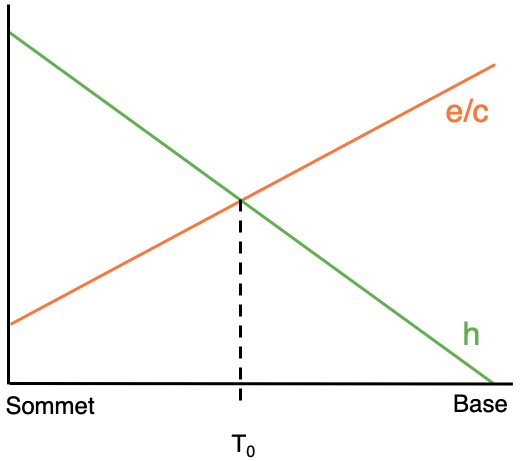
\includegraphics[height=.50\paperheight]{figs/modele1.png}}
    \only<2>{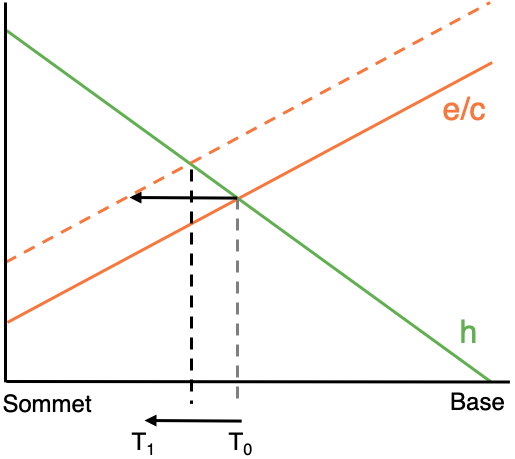
\includegraphics[height=.50\paperheight]{figs/modele2.png}}
    \only<3>{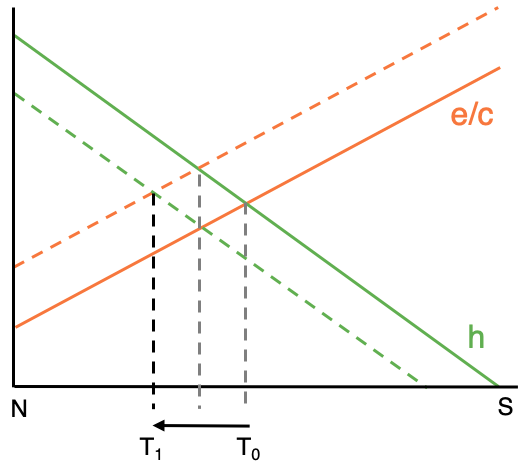
\includegraphics[height=.50\paperheight]{figs/modele3.png}}
  \end{figure}

\end{frame}

%% L'espèce à l'échelle régionale sera présente là où le ratio est suppérieur à la disponibilité de l'habitat (sa forêt)
%% Amène à une contraction de l'aire de distribution pour une espèce de sommet
%% Amène à une extension de l'aire de distribution pour un espèce associée à la base

%%%%%%%%%%%%%%%%%%%%%%%%%%%%%%%%%%%%%%%%%%%%%%%%%%%%%%%%%%%%%%%%%%%%%%%%%%%%%%%%%
% % %

\begin{frame}{Approche\hskip 1em \mdseries{\textcolor{lightgray}{Développer un outil théorique}}}

  2. Traduire le problème en un \textbf{modèle mathématique} de métapopulation qui tiendra compte de \emph{l'aire} des patchs, de \emph{la distance inter-patch} et \emph{du climat} dans les patchs

  %\begin{equation*}
  %  \frac{dP_i}{dt} = c(T_i) \sum{exp(-\alpha d_ij)} f(T_j,A_j)(1-P_i) - e(T_i,A_i)P_i
  %\end{equation*}

  \begin{figure}
    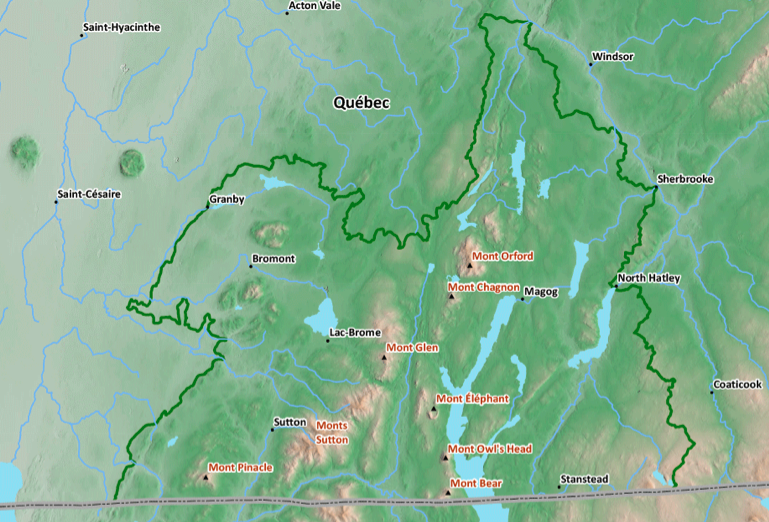
\includegraphics[height=.55\paperheight]{figs/appalaches.png}
  \end{figure}

\end{frame}

%% Modèle réalistique (spatiallement explicite)
%% Une équation pour la probabilité que chaque patch soit occuppée
%% Prend en compte la distribution spatiale des patchs (montagnes) (aire, distance), le climat de chaque patch et la dispersion de l'espèce
%%

%%%%%%%%%%%%%%%%%%%%%%%%%%%%%%%%%%%%%%%%%%%%%%%%%%%%%%%%%%%%%%%%%%%%%%%%%%%%%%%%%
% % %

\begin{frame}{Approche\hskip 1em \mdseries{\textcolor{lightgray}{L'impact des interactions}}}

  3. Mesurer la \textbf{capacité de support} de la métapopulation

  % Figure du range (métapop) de l'espèce avant et après changement climatique

\end{frame}

%% Objectif: mesurer l'impact sur l'ampleur de la réponse à l'échelle régionale (à l'échelle de la métapop)
%% En regardant le degré de réponse de l'habitat, l'effet des interactions sur la réponse pourra être observée sur le risque d'extinction de l'espèce apres changement climatique

%%%%%%%%%%%%%%%%%%%%%%%%%%%%%%%%%%%%%%%%%%%%%%%%%%%%%%%%%%%%%%%%%%%%%%%%%%%%%%%%%
% % %

\begin{frame}{Approche\hskip 1em \mdseries{\textcolor{lightgray}{L'impact des interactions}}}

  4. Mesurer la \textbf{vitesse de réaction} de la métapopulation



\end{frame}

%% Objectif: mesurer l'impact sur la dynamique de la réponse; de la sensibilité de l'espèce auc c.c.

%%%%%%%%%%%%%%%%%%%%%%%%%%%%%%%%%%%%%%%%%%%%%%%%%%%%%%%%%%%%%%%%%%%%%%%%%%%%%%%%%
% % %

\begin{frame}{Contributions\hskip 1em \mdseries{\textcolor{lightgray}{}}}

  Mon travail contribuera à:

  \begin{itemize}
    \item Une meilleure compréhension de \textbf{l'effet des interactions} sur la réponse des espèces face au changement climatique;
    \item Produira des \textbf{hypothèses} qui pourront être vérifiées sur le terrain;
    \item Aidera Corridor Appalachien à \textbf{documenter le futur} des sommets de conifères et de certaines espèces;
  \end{itemize}

\end{frame}

%% Mon travail amènera une meilleure compréhension de l'effet des interactions sur la réponse des espèces face au changement climatique qui était ingnorée des modèles de distribution d'espèce classiques alors qu'il y a d'importantes preuves de leur effet.

%%%%%%%%%%%%%%%%%%%%%%%%%%%%%%%%%%%%%%%%%%%%%%%%%%%%%%%%%%%%%%%%%%%%%%%%%%%%%%%%%
% % %

\begin{frame}{Remerciements\hskip 1em \mdseries{\textcolor{lightgray}{}}}

  \begin{columns}
    \begin{column}{0.5\textwidth}
      Dominique Gravel

      Mark Velend
      Marc Bélisle
      Anna Hargreaves
    \end{column}

    \begin{column}{0.5\textwidth}
      Membres du laboratoire Gravel

      Guillaume blanchet
    \end{column}
  \end{columns}

\end{frame}

%% Mon travail amènera une meilleure compréhension de l'effet des interactions sur la réponse des espèces face au changement climatique qui était ingnorée des modèles de distribution d'espèce classiques alors qu'il y a d'importantes preuves de leur effet.

%%%%%%%%%%%%%%%%%%%%%%%%%%%%%%%%%%%%%%%%%%%%%%%%%%%%%%%%%%%%%%%%%%%%%%%%%%%%%%%%%
% % %

\begin{frame}[standout]

  Questions?

\end{frame}

%% Mon travail amènera une meilleure compréhension de l'effet des interactions sur la réponse des espèces face au changement climatique qui était ingnorée des modèles de distribution d'espèce classiques alors qu'il y a d'importantes preuves de leur effet.

%%%%%%%%%%%%%%%%%%%%%%%%%%%%%%%%%%%%%%%%%%%%%%%%%%%%%%%%%%%%%%%%%%%%%%%%%%%%%%%%%
% % %
\appendix

\begin{frame}{Appendice\hskip 1em \mdseries{\textcolor{lightgray}{Modèle mathématique}}}{Backup slides}

  Modèle spatiallement explicite de métapopulation

  \begin{equation*}
    \frac{dP_i}{dt} = c(T_i) \sum{exp(-\alpha d_ij)} f(T_j,A_j)(1-P_i) - e(T_i,A_i)P_i
  \end{equation*}

  \begin{figure}
    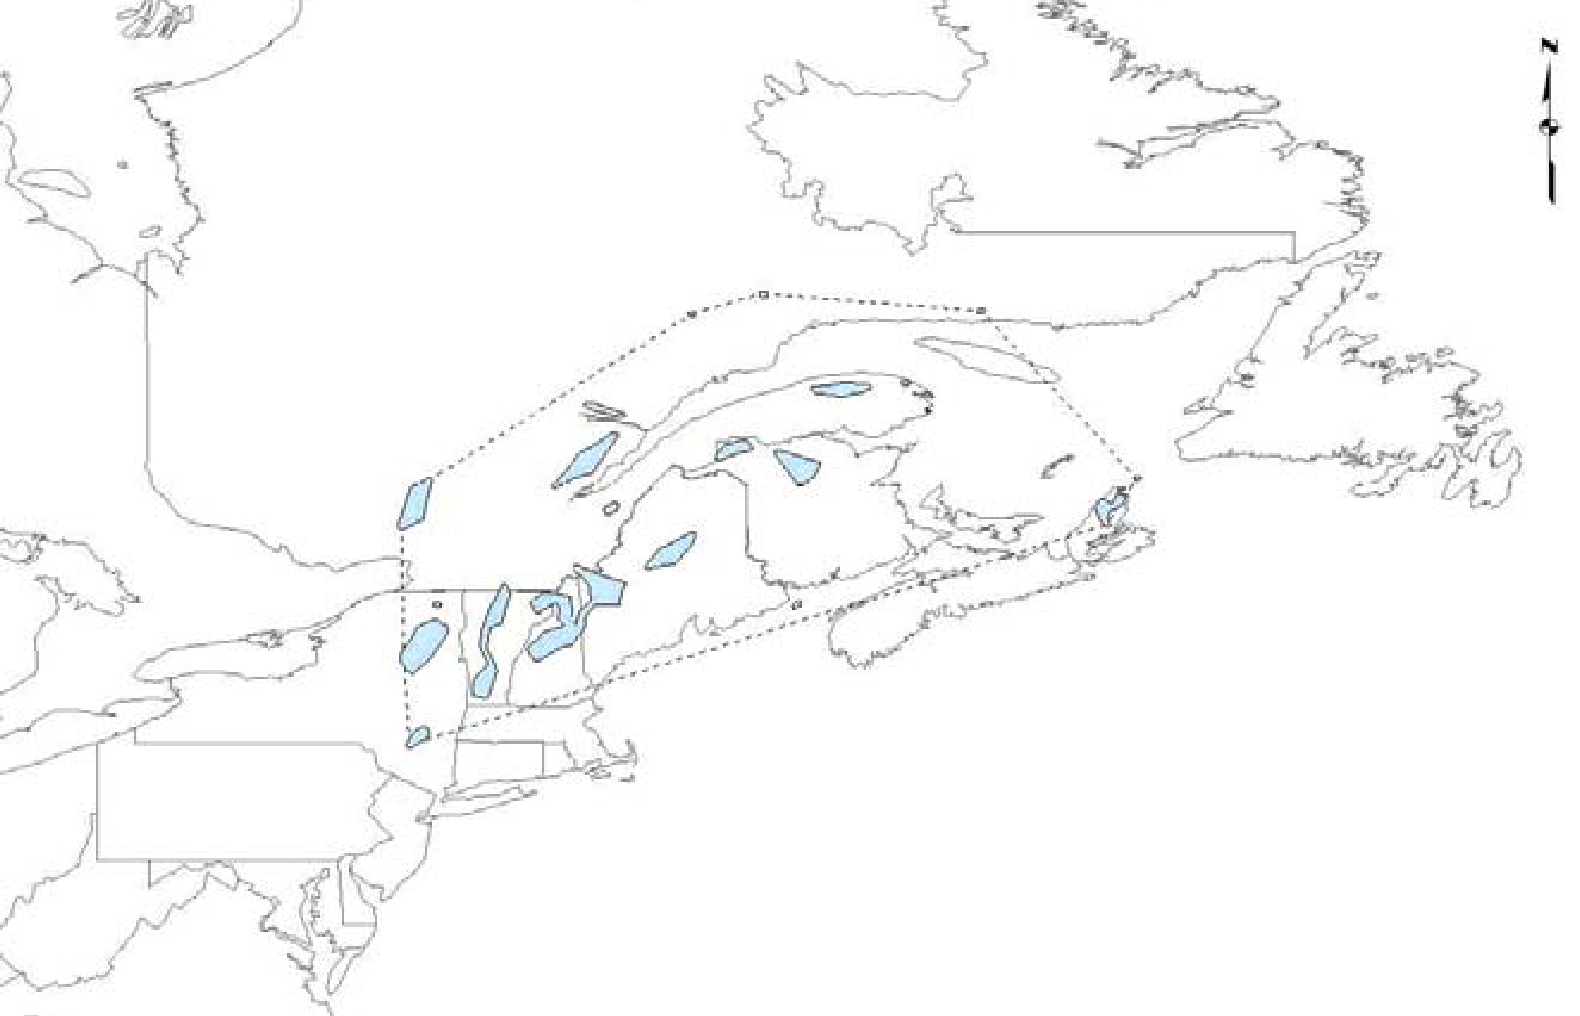
\includegraphics[height=.50\paperheight]{figs/grive.png}
  \end{figure}

\end{frame}

%%%%%%%%%%%%%%%%%%%%%%%%%%%%%%%%%%%%%%%%%%%%%%%%%%%%%%%%%%%%%%%%%%%%%%%%%%%%%%%%%
% % %

{%
\setbeamertemplate{frame footer}{Svenning \textit{et al}. 2014}
\begin{frame}{Théorie\hskip 1em \mdseries{\textcolor{lightgray}{Range shifts}}}

  \begin{figure}
  	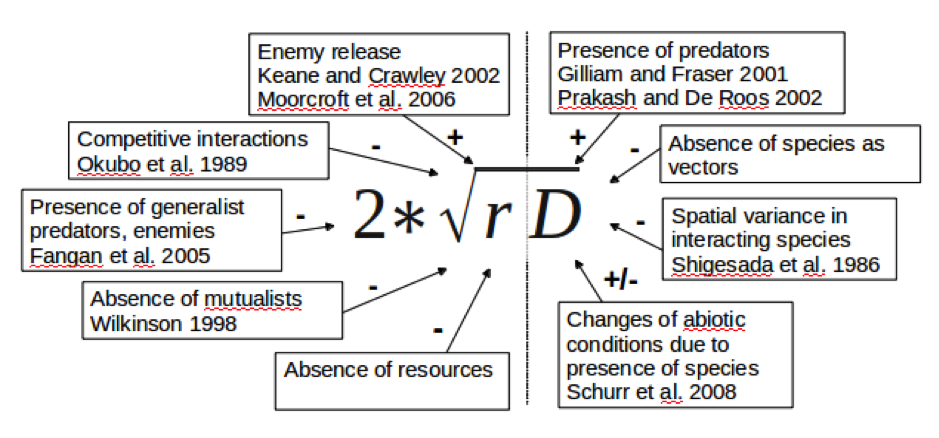
\includegraphics[height=.65\paperheight]{figs/svenning.png}
    %\caption*{ \textbf{}}
  \end{figure}

\end{frame}
}

%%%%%%%%%%%%%%%%%%%%%%%%%%%%%%%%%%%%%%%%%%%%%%%%%%%%%%%%%%%%%%%%%%%%%%%%%%%%%%%%%

\end{document}
